% !Mode:: "TeX:UTF-8"
% !TEX encoding = UTF-8 Unicode

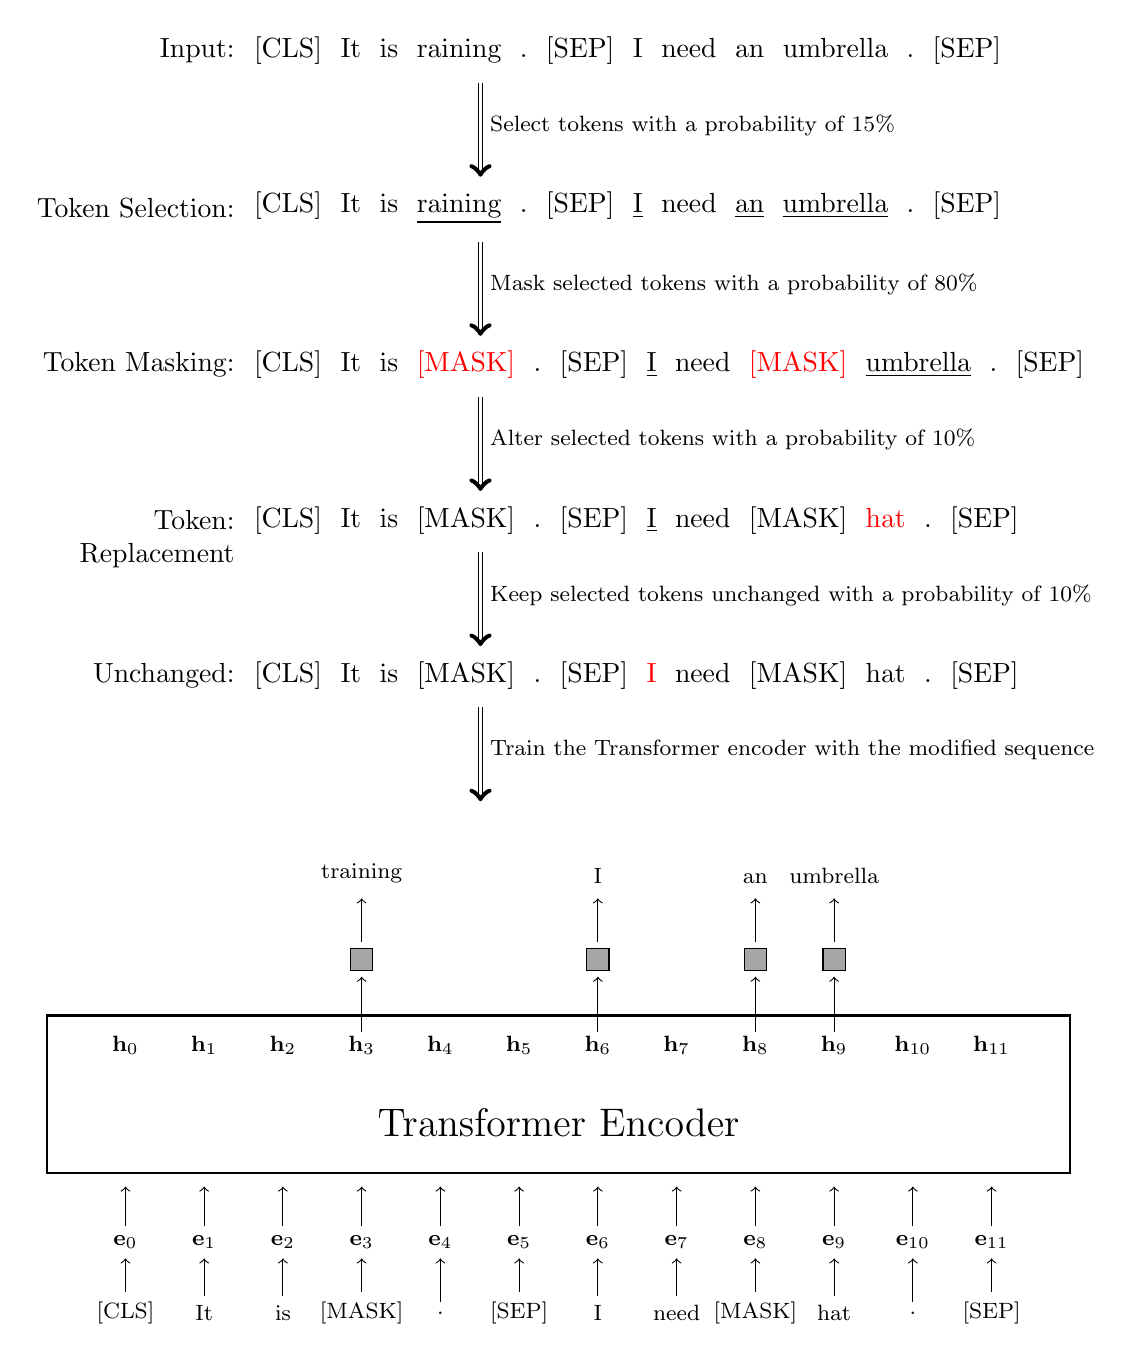
\begin{tikzpicture}
	
\def\vstep{1.3cm}
\def\ssep{1.0cm}

\tikzstyle{enode} = [minimum width=9*\nodestep,minimum height=1.4*\nodestep,inner sep=2pt,draw,thick];

\begin{scope}

%%%%%% input
\node [anchor=west] (original) at (0,0) {$[\mathrm{CLS}]$\ \ It\ \ is\ \ raining\ \ .\ \ $[\mathrm{SEP}]$\ \ I\ \ need\ \ an\ \ umbrella\ \ .\ \ $[\mathrm{SEP}]$};
\node [anchor=east] (originalcaption) at ([xshift=-0.0em]original.west) {Input:};

\draw [->,double,double distance=1pt] ([xshift=3cm,yshift=-3pt]original.south west) -- ([xshift=3cm,yshift=-\vstep]original.south west);
\node [anchor=west] (step0) at ([xshift=3cm,yshift=-0.5*\vstep]original.south west) {\footnotesize{Select tokens with a probability of $15\%$}};

%%%%%% selected tokens
\node [anchor=north west] (selected) at ([yshift=-\vstep-0.2em]original.south west) {$[\mathrm{CLS}]$\ \ It\ \ is\ \ \underline{raining}\ \ .\ \ $[\mathrm{SEP}]$\ \ \underline{I}\ \ need\ \ \underline{an}\ \ \underline{umbrella}\ \ .\ \ $[\mathrm{SEP}]$};
\node [anchor=east] (selectedcaption) at ([xshift=-0.0em]selected.west) {Token Selection:};

\draw [->,double,double distance=1pt] ([xshift=3cm,yshift=-3pt]selected.south west) -- ([xshift=3cm,yshift=-\vstep]selected.south west);
\node [anchor=west] (step1) at ([xshift=3cm,yshift=-0.5*\vstep]selected.south west) {\footnotesize{Mask selected tokens with a probability of $80\%$}};

%%%%%% masked tokens
\node [anchor=north west] (masked) at ([yshift=-\vstep-0.2em]selected.south west) {$[\mathrm{CLS}]$\ \ It\ \ is\ \ {\color{red} $\mathrm{[MASK]}$}\ \ .\ \ $[\mathrm{SEP}]$\ \ \underline{I}\ \ need\ \ {\color{red} $\mathrm{[MASK]}$}\ \ \underline{umbrella}\ \ .\ \ $[\mathrm{SEP}]$};
\node [anchor=east] (maskedcaption) at ([xshift=-0.0em]masked.west) {Token Masking:};

\draw [->,double,double distance=1pt] ([xshift=3cm,yshift=-3pt]masked.south west) -- ([xshift=3cm,yshift=-\vstep]masked.south west);
\node [anchor=west] (step2) at ([xshift=3cm,yshift=-0.5*\vstep]masked.south west) {\footnotesize{Alter selected tokens with a probability of $10\%$}};

%%%%%% replaced tokens
\node [anchor=north west] (replaced) at ([yshift=-\vstep-0.2em]masked.south west) {$[\mathrm{CLS}]$\ \ It\ \ is\ \ $\mathrm{[MASK]}$\ \ .\ \ $[\mathrm{SEP}]$\ \ \underline{I}\ \ need\ \ $\mathrm{[MASK]}$\ \ {\color{red} hat}\ \ .\ \ $[\mathrm{SEP}]$};
\node [anchor=east] (replacedcaption) at ([xshift=-0.0em]replaced.west) {Token:};
\node [anchor=north east] (replacedcaption2) at ([yshift=2pt]replacedcaption.south east) {Replacement};

\draw [->,double,double distance=1pt] ([xshift=3cm,yshift=-3pt]replaced.south west) -- ([xshift=3cm,yshift=-\vstep]replaced.south west);
\node [anchor=west] (step3) at ([xshift=3cm,yshift=-0.5*\vstep]replaced.south west) {\footnotesize{Keep selected tokens unchanged with a probability of $10\%$}};

%%%%%% unchanged tokens
\node [anchor=north west] (unchanged) at ([yshift=-\vstep-0.2em]replaced.south west) {$[\mathrm{CLS}]$\ \ It\ \ is\ \ $\mathrm{[MASK]}$\ \ .\ \ $[\mathrm{SEP}]$\ \ {\color{red} I}\ \ need\ \ $\mathrm{[MASK]}$\ \ hat\ \ .\ \ $[\mathrm{SEP}]$};
\node [anchor=east] (unchangedcaption) at ([xshift=-0.0em]unchanged.west) {Unchanged:};

\draw [->,double,double distance=1pt] ([xshift=3cm,yshift=-3pt]unchanged.south west) -- ([xshift=3cm,yshift=-\vstep]unchanged.south west);
\node [anchor=west] (step4) at ([xshift=3cm,yshift=-0.5*\vstep]unchanged.south west) {\footnotesize{Train the Transformer encoder with the modified sequence}};

%%%%%% train the encoder

\node [anchor=west] (w0) at ([yshift=-6*\vstep,xshift=-2cm]unchanged.south west) {\footnotesize{$[\mathrm{CLS}]$}};
\node [anchor=center] (w1) at ([xshift=\ssep]w0.center) {\footnotesize{It}};
\node [anchor=center] (w2) at ([xshift=\ssep]w1.center) {\footnotesize{is}};
\node [anchor=center] (w3) at ([xshift=\ssep]w2.center) {\footnotesize{$\mathrm{[MASK]}$}};
\node [anchor=center] (w4) at ([xshift=\ssep]w3.center) {\footnotesize{.}};
\node [anchor=center] (w5) at ([xshift=\ssep]w4.center) {\footnotesize{$\mathrm{[SEP]}$}};
\node [anchor=center] (w6) at ([xshift=\ssep]w5.center) {\footnotesize{I}};
\node [anchor=center] (w7) at ([xshift=\ssep]w6.center) {\footnotesize{need}};
\node [anchor=center] (w8) at ([xshift=\ssep]w7.center) {\footnotesize{$\mathrm{[MASK]}$}};
\node [anchor=center] (w9) at ([xshift=\ssep]w8.center) {\footnotesize{hat}};
\node [anchor=center] (w10) at ([xshift=\ssep]w9.center) {\footnotesize{.}};
\node [anchor=center] (w11) at ([xshift=\ssep]w10.center) {\footnotesize{$\mathrm{[SEP]}$}};

\node [anchor=center] (e0) at ([yshift=0.9*\ssep]w0.center) {\footnotesize{$\mathbf{e}_0$}};
\node [anchor=center] (e1) at ([yshift=0.9*\ssep]w1.center) {\footnotesize{$\mathbf{e}_1$}};
\node [anchor=center] (e2) at ([yshift=0.9*\ssep]w2.center) {\footnotesize{$\mathbf{e}_2$}};
\node [anchor=center] (e3) at ([yshift=0.9*\ssep]w3.center) {\footnotesize{$\mathbf{e}_3$}};
\node [anchor=center] (e4) at ([yshift=0.9*\ssep]w4.center) {\footnotesize{$\mathbf{e}_4$}};
\node [anchor=center] (e5) at ([yshift=0.9*\ssep]w5.center) {\footnotesize{$\mathbf{e}_5$}};
\node [anchor=center] (e6) at ([yshift=0.9*\ssep]w6.center) {\footnotesize{$\mathbf{e}_6$}};
\node [anchor=center] (e7) at ([yshift=0.9*\ssep]w7.center) {\footnotesize{$\mathbf{e}_7$}};
\node [anchor=center] (e8) at ([yshift=0.9*\ssep]w8.center) {\footnotesize{$\mathbf{e}_8$}};
\node [anchor=center] (e9) at ([yshift=0.9*\ssep]w9.center) {\footnotesize{$\mathbf{e}_9$}};
\node [anchor=center] (e10) at ([yshift=0.9*\ssep]w10.center) {\footnotesize{$\mathbf{e}_{10}$}};
\node [anchor=center] (e11) at ([yshift=0.9*\ssep]w11.center) {\footnotesize{$\mathbf{e}_{11}$}};

\draw [->] (w0.north) -- (e0.south);
\draw [->] (w1.north) -- (e1.south);
\draw [->] (w2.north) -- (e2.south);
\draw [->] (w3.north) -- (e3.south);
\draw [->] (w4.north) -- (e4.south);
\draw [->] (w5.north) -- (e5.south);
\draw [->] (w6.north) -- (e6.south);
\draw [->] (w7.north) -- (e7.south);
\draw [->] (w8.north) -- (e8.south);
\draw [->] (w9.north) -- (e9.south);
\draw [->] (w10.north) -- (e10.south);
\draw [->] (w11.north) -- (e11.south);

\draw [->] (e0.north) -- ([yshift=0.5*\ssep]e0.north);
\draw [->] (e1.north) -- ([yshift=0.5*\ssep]e1.north);
\draw [->] (e2.north) -- ([yshift=0.5*\ssep]e2.north);
\draw [->] (e3.north) -- ([yshift=0.5*\ssep]e3.north);
\draw [->] (e4.north) -- ([yshift=0.5*\ssep]e4.north);
\draw [->] (e5.north) -- ([yshift=0.5*\ssep]e5.north);
\draw [->] (e6.north) -- ([yshift=0.5*\ssep]e6.north);
\draw [->] (e7.north) -- ([yshift=0.5*\ssep]e7.north);
\draw [->] (e8.north) -- ([yshift=0.5*\ssep]e8.north);
\draw [->] (e9.north) -- ([yshift=0.5*\ssep]e9.north);
\draw [->] (e10.north) -- ([yshift=0.5*\ssep]e10.north);
\draw [->] (e11.north) -- ([yshift=0.5*\ssep]e11.north);

\node [anchor=south,minimum width=13*\ssep,minimum height=2*\ssep,draw,thick] (encoder) at ([yshift=1.5*\ssep,xshift=0.5*\ssep]w5.north) {};

\node [anchor=center] (h0) at ([yshift=3.4*\ssep]w0.center) {\footnotesize{$\mathbf{h}_0$}};
\node [anchor=center] (h1) at ([yshift=3.4*\ssep]w1.center) {\footnotesize{$\mathbf{h}_1$}};
\node [anchor=center] (h2) at ([yshift=3.4*\ssep]w2.center) {\footnotesize{$\mathbf{h}_2$}};
\node [anchor=center] (h3) at ([yshift=3.4*\ssep]w3.center) {\footnotesize{$\mathbf{h}_3$}};
\node [anchor=center] (h4) at ([yshift=3.4*\ssep]w4.center) {\footnotesize{$\mathbf{h}_4$}};
\node [anchor=center] (h5) at ([yshift=3.4*\ssep]w5.center) {\footnotesize{$\mathbf{h}_5$}};
\node [anchor=center] (h6) at ([yshift=3.4*\ssep]w6.center) {\footnotesize{$\mathbf{h}_6$}};
\node [anchor=center] (h7) at ([yshift=3.4*\ssep]w7.center) {\footnotesize{$\mathbf{h}_7$}};
\node [anchor=center] (h8) at ([yshift=3.4*\ssep]w8.center) {\footnotesize{$\mathbf{h}_8$}};
\node [anchor=center] (h9) at ([yshift=3.4*\ssep]w9.center) {\footnotesize{$\mathbf{h}_9$}};
\node [anchor=center] (h10) at ([yshift=3.4*\ssep]w10.center) {\footnotesize{$\mathbf{h}_{10}$}};
\node [anchor=center] (h11) at ([yshift=3.4*\ssep]w11.center) {\footnotesize{$\mathbf{h}_{11}$}};

\node [anchor=south,minimum height=0.8em,minimum width=0.8em,draw,fill=gray!70] (s3) at ([yshift=0.7*\ssep]h3.north) {};
\node [anchor=south,minimum height=0.8em,minimum width=0.8em,draw,fill=gray!70] (s6) at ([yshift=0.7*\ssep]h6.north) {};
\node [anchor=south,minimum height=0.8em,minimum width=0.8em,draw,fill=gray!70] (s8) at ([yshift=0.7*\ssep]h8.north) {};
\node [anchor=south,minimum height=0.8em,minimum width=0.8em,draw,fill=gray!70] (s9) at ([yshift=0.7*\ssep]h9.north) {};

\draw [->] ([yshift=-2pt]h3.north) -- ([yshift=-2pt]s3.south);
\draw [->] ([yshift=-2pt]h6.north) -- ([yshift=-2pt]s6.south);
\draw [->] ([yshift=-2pt]h8.north) -- ([yshift=-2pt]s8.south);
\draw [->] ([yshift=-2pt]h9.north) -- ([yshift=-2pt]s9.south);

\node [anchor=south] (o3) at ([yshift=0.7*\ssep]s3.north) {\footnotesize{training}};
\node [anchor=south] (o6) at ([yshift=0.7*\ssep]s6.north) {\footnotesize{I}};
\node [anchor=south] (o8) at ([yshift=0.7*\ssep,xshift=0.0em]s8.north) {\footnotesize{an}};
\node [anchor=south] (o9) at ([yshift=0.7*\ssep,xshift=0.0em]s9.north) {\footnotesize{umbrella}};

\draw [->] ([yshift=2pt]s3.north) -- ([yshift=0.7*\ssep-2pt]s3.north);
\draw [->] ([yshift=2pt]s6.north) -- ([yshift=0.7*\ssep-2pt]s6.north);
\draw [->] ([yshift=2pt]s8.north) -- ([yshift=0.7*\ssep-2pt]s8.north);
\draw [->] ([yshift=2pt]s9.north) -- ([yshift=0.7*\ssep-2pt]s9.north);

\node [anchor=south] (encodercaption) at ([yshift=1em]encoder.south) {\Large{Transformer Encoder}};

\end{scope}
	
\end{tikzpicture}
